\section{Zeitablauf}
\subsection{Gantt-Chart}
Ein Gantt-Diagramm oder auch Balkenplan ist ein Instrument des Projektmanagements, das die zeitliche Abfolge von Aktivitäten grafisch in Form von Balken auf einer Zeitachse darstellt.
\\\\
In den unteren Abbildungen sieht man einerseits die einzelnen Aktivitäten, Ressourcen und die Mitarbeiter die wir für unser Projekt "`Roboter-Fangen"' eingeplant haben, einmal als Liste und in einer grafischen Darstellung.

Außerdem kann man in der Liste erkennen, welche Aktivität welchen Vorgänger bzw. Nachfolger hat. Wo von es abhängig ist. 

Durch die grafische Darstellung ist es möglich frühzeitig Engpässe zu erkennen und das Projekt nötigen falls um zu strukturieren.
\\\\
Einige Aktivitäten haben wir der Übersichtlichkeit in Gruppen eingeteilt:\\\\
\begin{tabular}{p{0.5\textwidth}p{0.5\textwidth}}
	\textbf{Gruppen:} & \textbf{Meilensteine:}\\
	\begin{itemize}
		\item Planung
		\item Programmierung-Teil 1
		\begin{itemize}
			\item Simple KI
		\end{itemize}
		\item Programmierung-Teil 2
		\item Dokumentation
	\end{itemize} & 
	\begin{itemize}
		\item M0: Start
		\item M1: Planung abgeschlossen
		\item M2: Erste Implementierung
		\item M3: Kurzpräsentation
		\item M4: Programmierung abgeschlossen
		\item M5: Endpräsentation
		\item M6: Dokumentation abgeschlossen
	\end{itemize}\\
\end{tabular}
\\
\begin{center}
		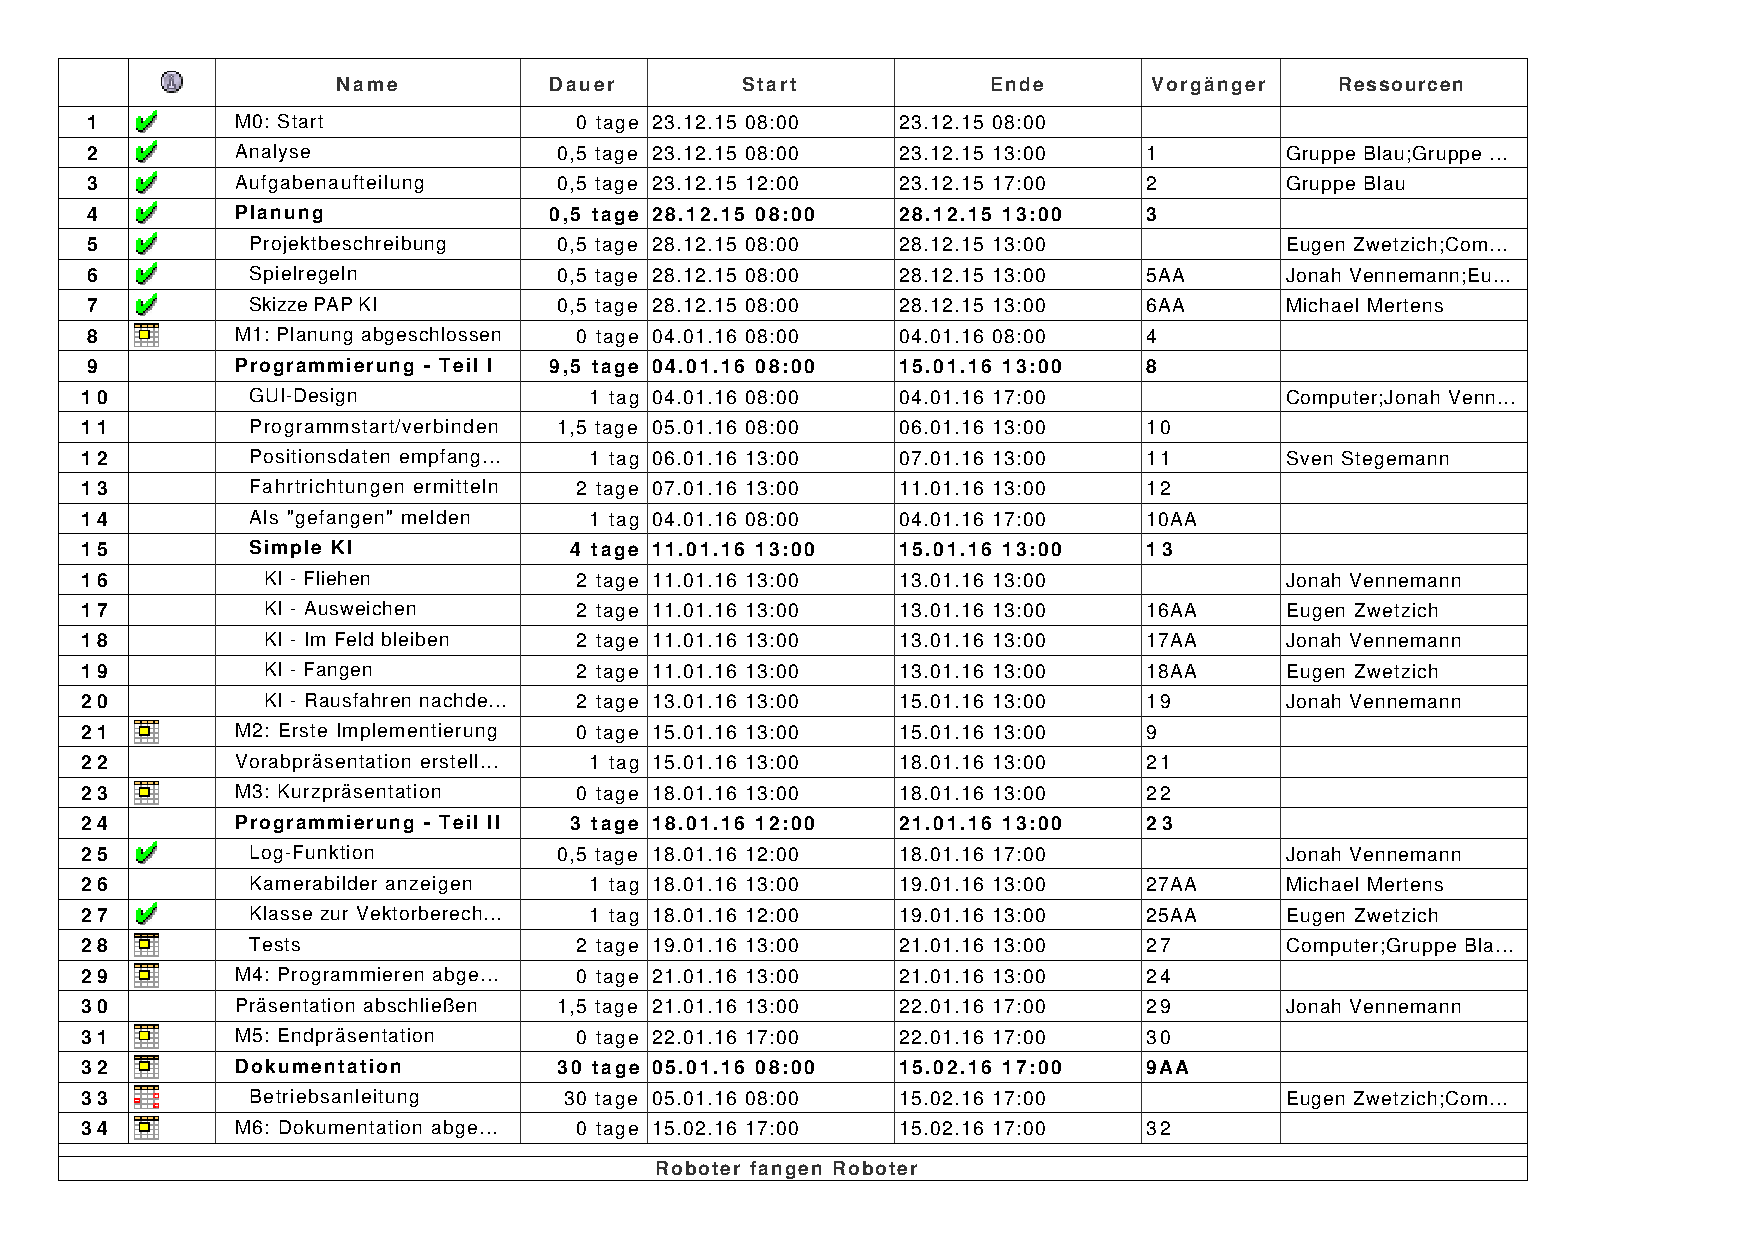
\includegraphics[width=0.8\textwidth]{Bilder/GanttDiagramm_[Page1].pdf}
		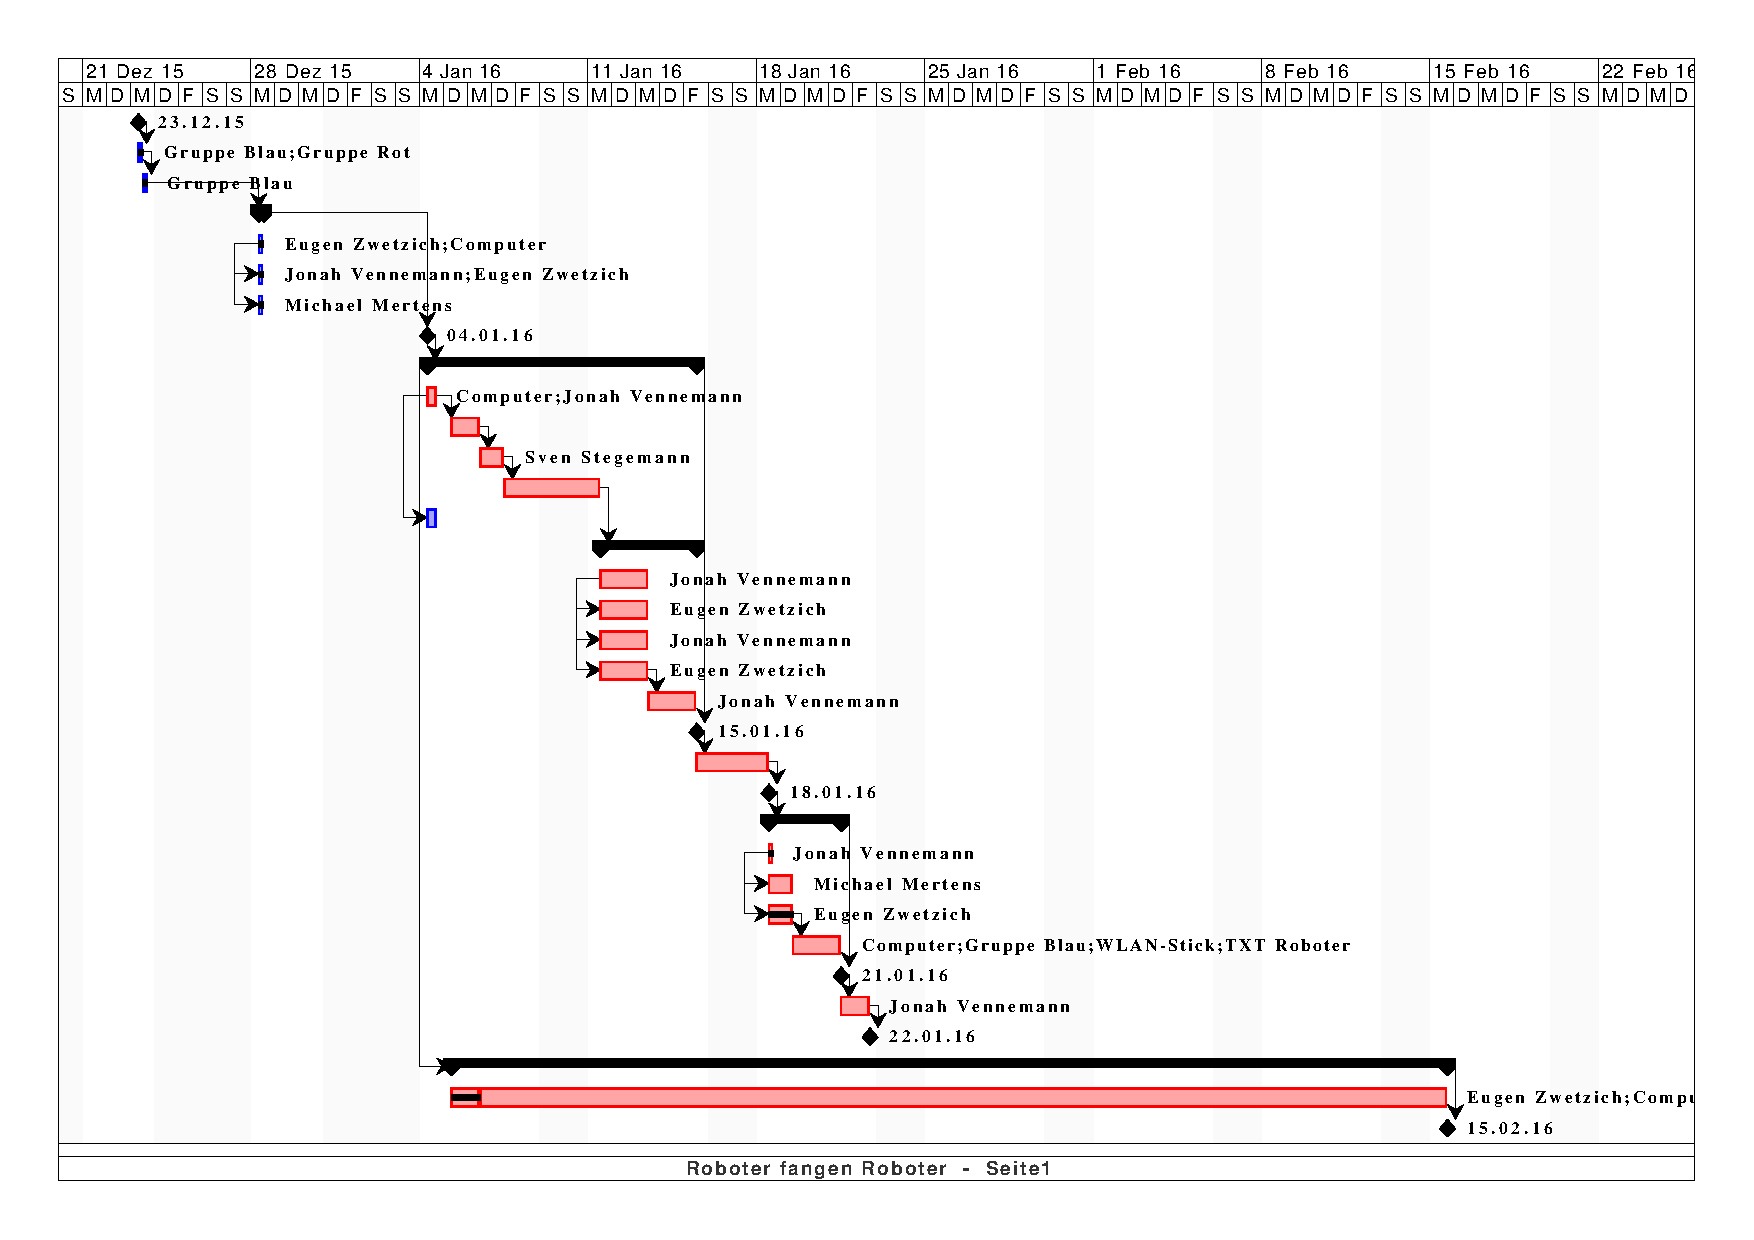
\includegraphics[width=0.8\textwidth]{Bilder/GanttDiagramm_[Page2].pdf}
		\captionof{figure}{Gantt-Chart v1.0}
\end{center}
\newpage
Aufgrund von Komplikationen mit den Roboter Klassen, mit dem Voranstreiten der Programmierung des Servers und der Komplexität der Programmierung der KI mussten wir die Planung des Projektes umstrukturieren.

Wir haben die Aktivitäten für die Benutzeroberfläche, das Ereignisprotokoll und die Vektorberechnung in den Programmierung-Teil 1 vorgezogen.

Erst im 2. Teil der Programmierung fingen wir mit der Programmierung der KI und der Kommunikation mit dem Server an.
\\\\
\textbf{Gruppen:} 
\begin{itemize}
	\item Planung
	\item Programmierung-Teil 1
	\item Programmierung-Teil 2
	\begin{itemize}
		\item Simple KI
	\end{itemize}
	\item Server-Team\\
\end{itemize} 
\textbf{Meilensteine:}
\begin{description}
	\item[M1: Planung abgeschlossen] Es muss die Projektbeschreibung, eine Skizze für die KI und ein Spielablauf fertig sein.
	\item[M2: Kurzpräsentation] Eine Präsentation über die zeitliche Planung und über die Aufwandsschätzung
	\item[M3: Programmierung abgeschlossen] Es muss die ganze Programmierung(Vektorberechnung, Künstliche Intelligenz, Benutzeroberfläche) der Software abgeschlossen sein. 
	\item[M4: Endpräsentation] Eine Abschlusspräsentation vom Projekt mit einer Vorführung des Spiels
	\item[M4: Dokumentation abgeschlossen] Abgabe der Dokumentation in ausgedruckter und digitaler Form
\end{description}

\begin{center}
	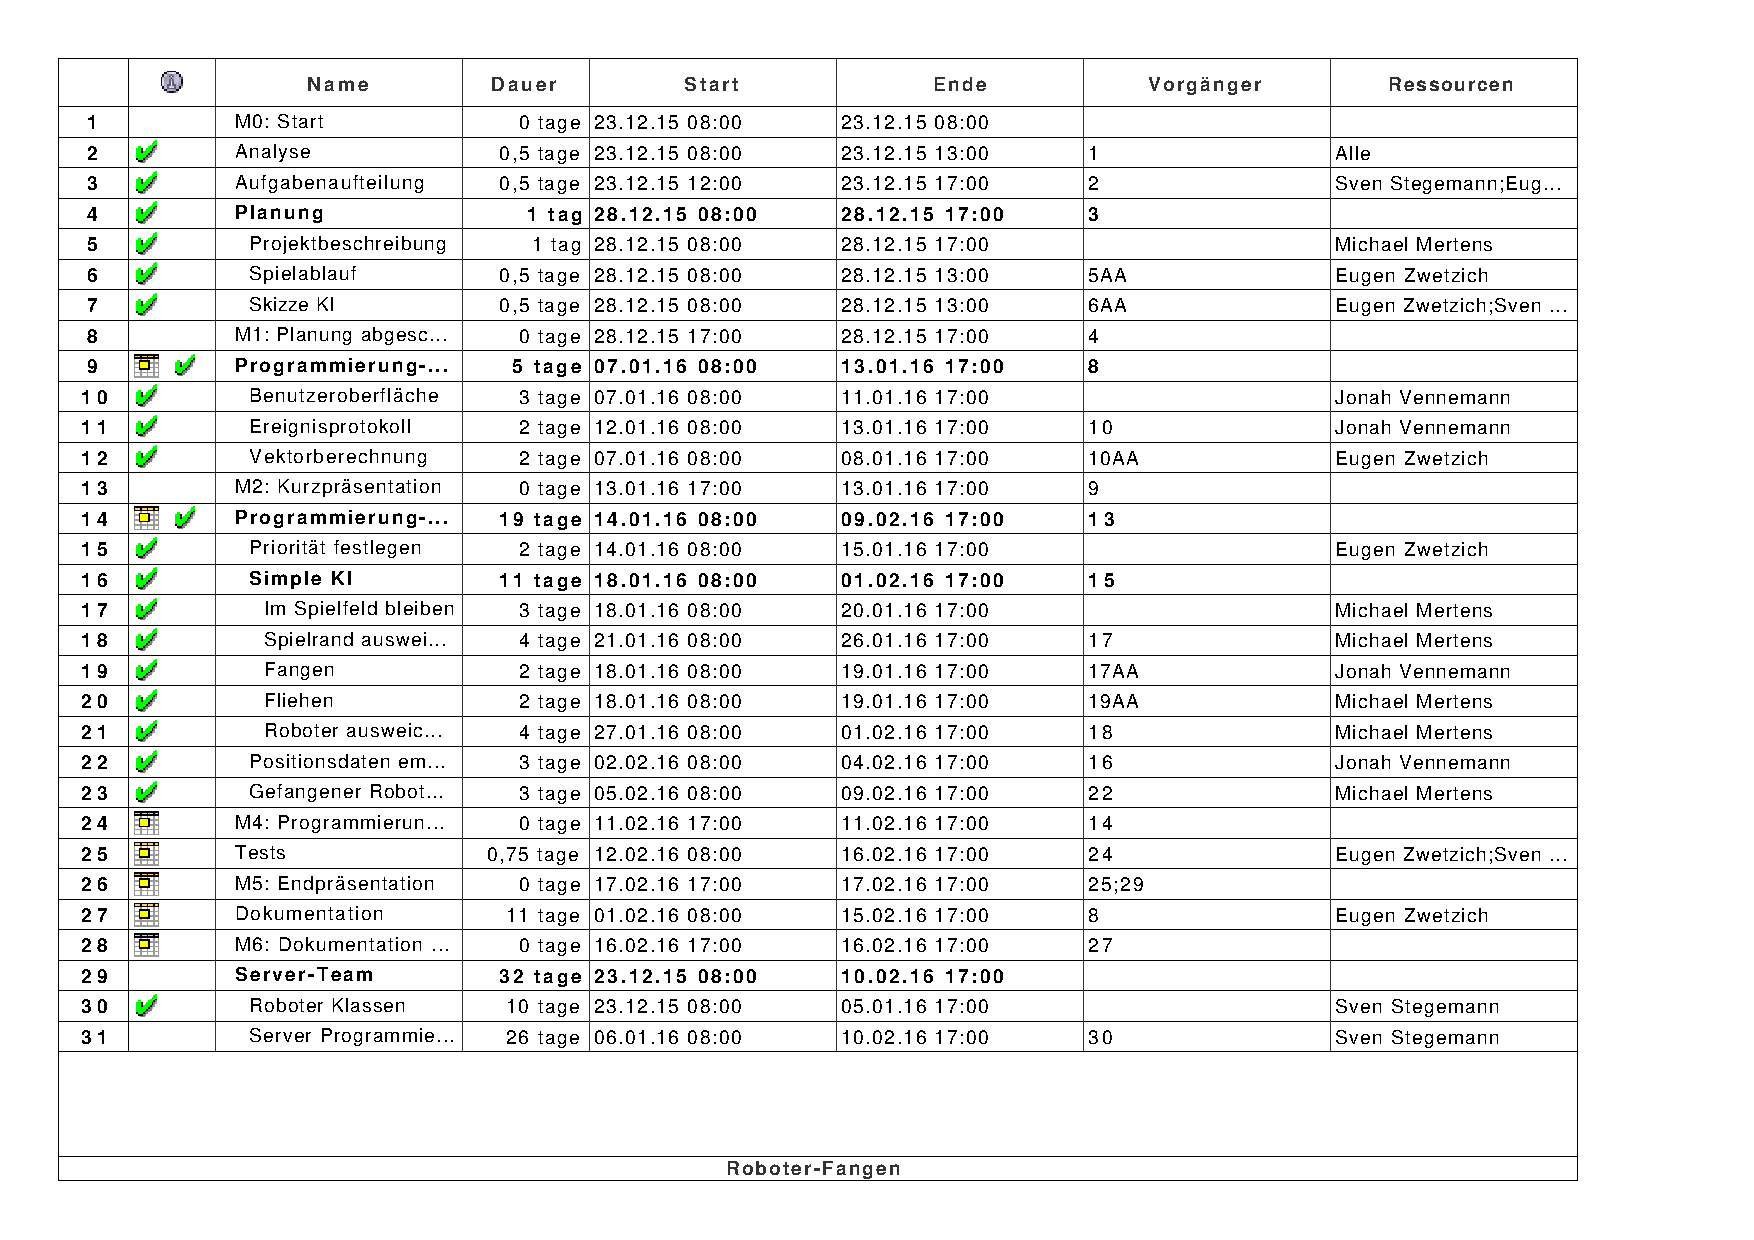
\includegraphics[width=0.8\textwidth]{Bilder/Roboter-Fangen_Liste.pdf}
	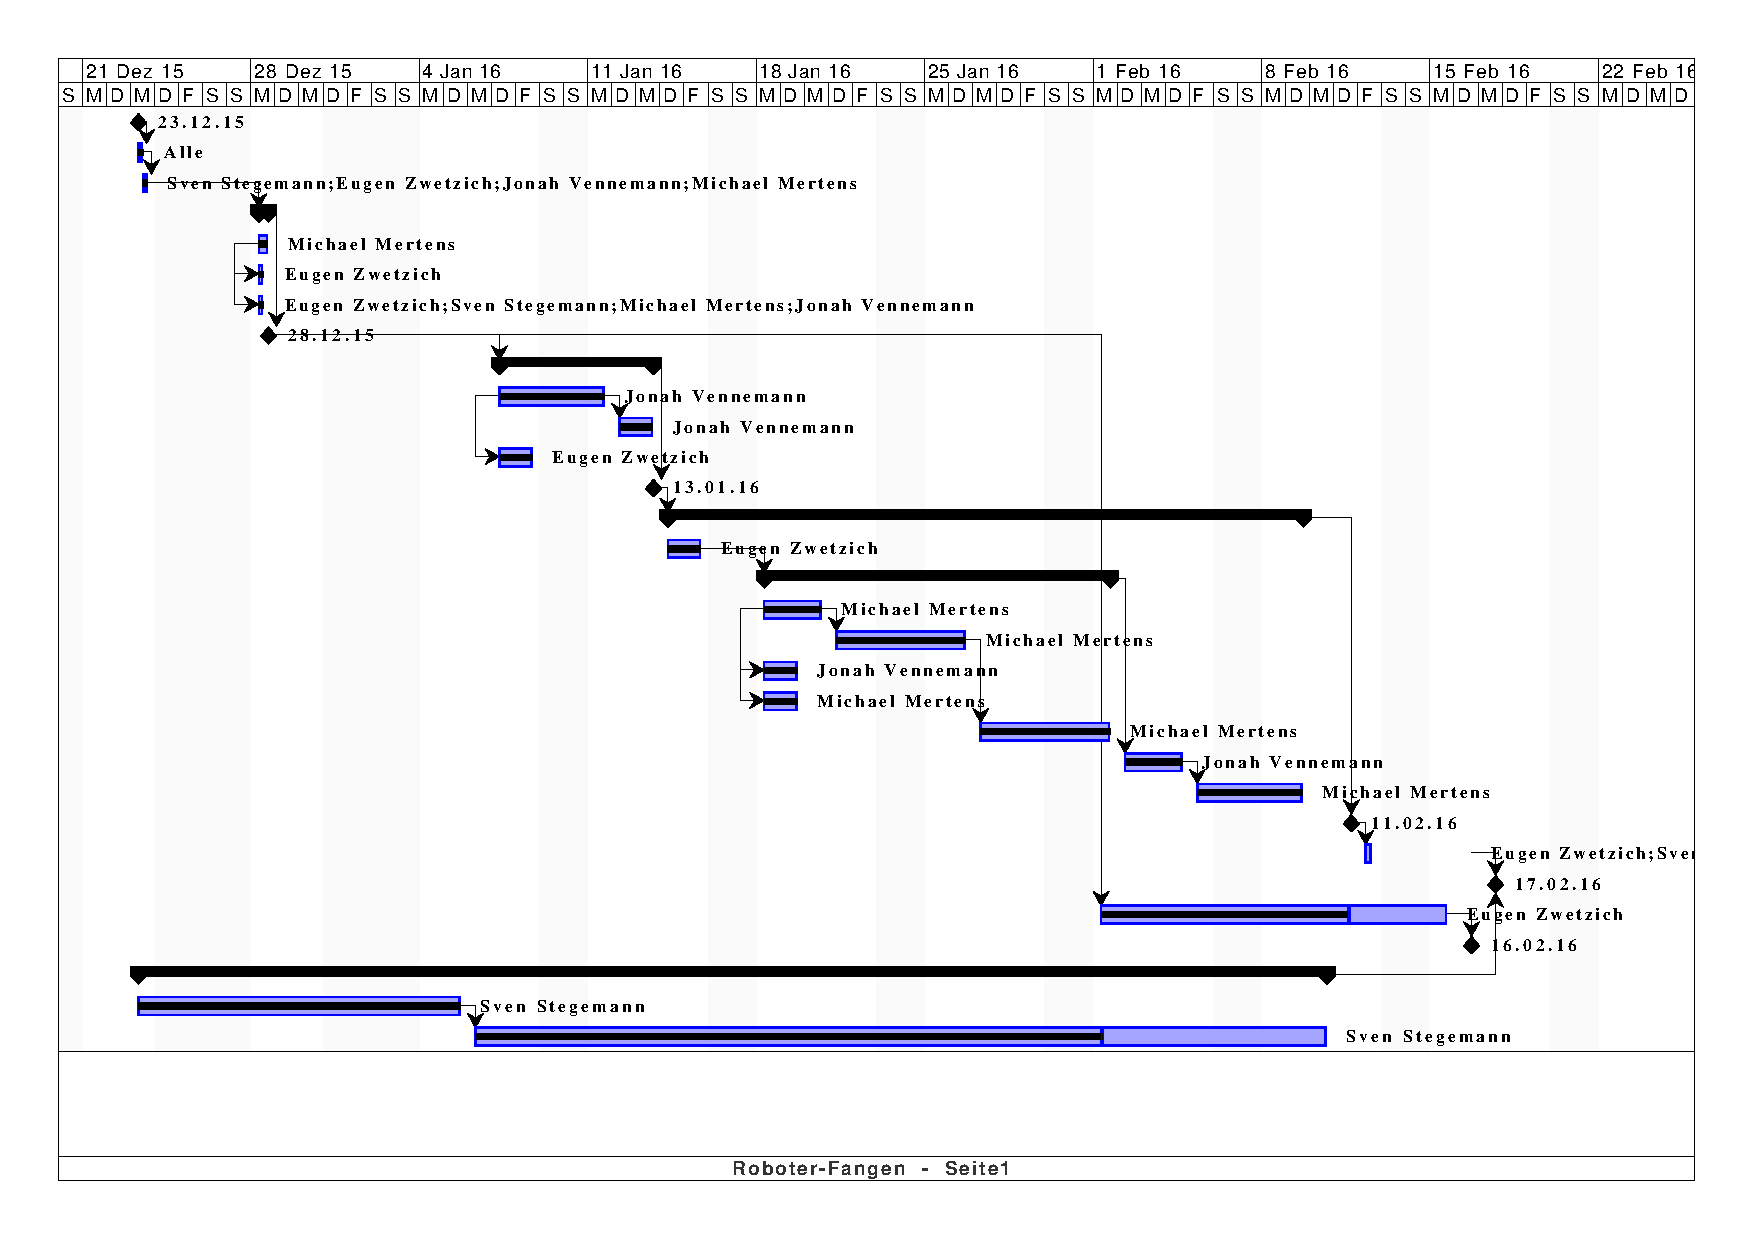
\includegraphics[width=0.8\textwidth]{Bilder/Roboter-Fangen_Grafik.pdf}
	\captionof{figure}{Gantt-Chart v2.0}
\end{center}
\newpage